\section{Quasi-stationary distribution}
\label{sec:qsd}

\cite{van2011quasi}. Both the BDC and BDK processes are subject to eventual
absorption --- either at the designated rupture state, or by death, at $0$.
But suppose there is an example of a particular realisation which has, by
chance, not yet reached fixation. It continues, increasingly against the
odds, as time marches on. How has it managed this? If it flies too low,
depletion to zero becomes more and more probable; but, almost as bad, if it
flies high, a population booming in number, there are all the more
opportunities for its downfall, a crashing and ceasing to be.
Like Icarus, the process which does not fall into the sea does so by
hovering at some appropriate height; its wings neither undermined by the
spray of a hungry ocean, nor by the beating rays of the sun at a rarified
altitude. \par
In such terms, we can examine this rogue process as it goes on to defy all
odds. Its fate will tend to be predicted by the quasi-stationary
distribution: a set of limiting conditional probabilities, each qualified by
non-fixation. \par

\subsection{Conditioning on survival}

Define the probability of fixation by time $t$: $F(t)$, whether by death or
collapse. This is settled immediately by the decomposition of \S2.4: a
realisation is fixed by $t$ precisely when it is not productively infected,
so
\begin{equation}
F(t)=1-\Ihat(t)=1-I(t)+D(t),
\end{equation}
which reduces to $F(t)=1-I(t)$ when $\mu=0$. The conditional state
probabilities decompose as
$$\pr{\xt = i} = \pr{\xt=i\mid \text{fixation}}F(t) + \pr{\xt=i\mid \text{non-fixation}} \lrb{1-F(t)}.$$
For $i\notin\{0,R\}$ the process has not been absorbed, so
$\pr{\xt=i\mid\text{fixation}}=0$, and it follows that
\begin{equation}
\pr{\xt=i\mid \text{non-fixation}} = \frac{p_i(t)}{1-F(t)}=\frac{p_i(t)}{\Ihat(t)}.
\label{eq:condp}
\end{equation}

The \emph{quasi-stationary distribution} (QSD) is the limiting form of these
conditional probabilities:
\begin{equation}
q_i:=\lim_{t\to\infty}\pr{\xt=i\mid\xt\notin\{0,R\}}
=\lim_{t\to\infty}\frac{p_i(t)}{\Ihat(t)},\qquad i\ge1.
\end{equation}

\subsection{The quasi-stationary distribution is geometric}

With the state probabilities \eqref{stateprob} in hand, the limit can be
taken explicitly. By \eqref{eq:condp} and \eqref{eq:pnsum},
$$
\pr{\xt=n\mid\xt\notin\{0,R\}}
=\frac{p_n(t)}{\sum_{m\ge1}p_m(t)}
=\lrb{1-P(t)}P(t)^{n-1},
$$
for every $t$. Since $P(t)\to1/a$ by \S\ref{sec:geometric-every-time}, the
limit exists and is explicit.

\begin{theorem}[Quasi-stationary distribution of the BDC]
\label{thm:qsd}
For all $\mu\ge0$, the quasi-stationary distribution of the BDC process is
geometric on $\{1,2,\ldots\}$ with ratio $1/a$:
\begin{equation}
q_n=\Bigl(1-\frac{1}{a}\Bigr)\Bigl(\frac{1}{a}\Bigr)^{n-1}
=(a-1)\,a^{-n},\qquad n\ge1.
\label{eq:qsd}
\end{equation}
\end{theorem}

Its moments follow at once:
\begin{equation}
\langle X\rangle_{\rm QS}=\frac{a}{a-1}=\frac{a}{A},
\qquad
\langle X^2\rangle_{\rm QS}=\frac{a(a+1)}{(a-1)^2},
\qquad
\mathrm{Var}_{\rm QS}(X)=\frac{a}{(a-1)^2}=\frac{a}{A^2}.
\label{eq:QSmoments}
\end{equation}
Observe that $\langle X\rangle_{\rm QS}=\mean{\Kb\mid\text{burst}}$ from
\eqref{eq:Vinf}, and that when $\mu=0$ both coincide with $V_\infty$ ---
the coincidence noted in \S\ref{sec:moments-recap}. For $\mu>0$ they differ:
at $(\beta,\mu,\delta)=(1,0.2,0.05)$, for example,
$\langle X\rangle_{\rm QS}\approx17.23$ while $V_\infty\approx13.99$.
Section~\S\ref{sec:burst-time-size} will give the reason: the burst size is
not merely equal in mean to the QS level --- the entire burst-size
distribution \emph{is} the quasi-stationary distribution.

\begin{figure}[H]
    \centering
    % First figure
    \begin{subfigure}{0.47\textwidth}
        \centering
        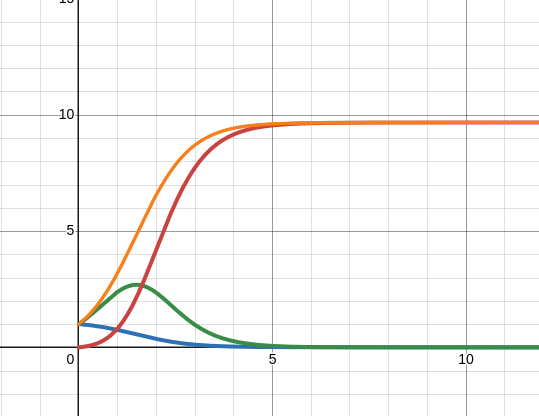
\includegraphics[width=\textwidth]{figures/IMG_ch5/QSmean/QS1} % Adjust the image path as necessary
        \caption{When $\mu = 0$.}
        \label{fig:figure1}
    \end{subfigure}
    \hspace{\fill} % Optional: adds space between figures
    % Second figure
    \begin{subfigure}{0.47\textwidth}
        \centering
        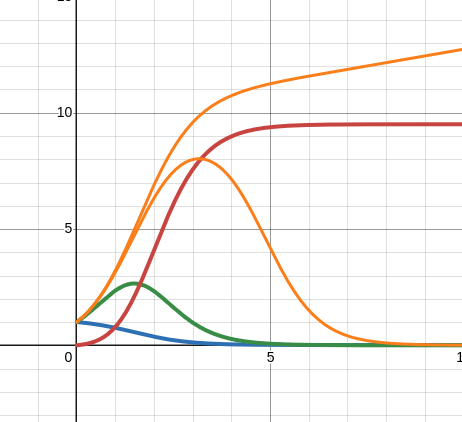
\includegraphics[width=\textwidth]{figures/IMG_ch5/QSmean/QS2} % Adjust the image path as necessary
        \caption{When $\mu > 0$.}
        \label{fig:figure2}
    \end{subfigure}

    \caption{Conditional means from simulation. (a) When $\mu=0$, the
    conditional mean $J(t)/I(t)$ tends to the same limit as $V(t)$, namely
    $1+\beta/\delta$. (b) When $\mu>0$, the curve rising at late time is the
    mean conditioned on non-fixation, $J(t)/\Ihat(t)$, tending to
    $\langle X\rangle_{\rm QS}=a/(a-1)$; the curve tending to $0$ is the mean
    conditioned only on non-catastrophe, $\mean{\xt\mid\xt\neq R}=J(t)/I(t)$,
    which vanishes because a fraction $b$ of realisations die out internally.}
    \label{fig:two_figures}
\end{figure}

Considering the no-death $\mu = 0$ case on the left above, it can be easily
seen that the conditional mean tends to the same limit as $V(t)$, which is
shown in red. That is
$$\lim_{t\to\infty}     \frac{J(t)}{I(t)}     =    \lim_{t\to\infty} V(t)  = 1 + \frac{\beta}{\delta}.$$
Here, when $\delta$ shrinks to $0$, the QS mean and expected release count
tend to infinity.

\subsection{Mean productive lifetime}
\label{sec:lifetime}

Before leaving the single-cell description, one more integral will be needed
in \S\ref{sec:peff-section}. The expected duration of productive infection
is
\begin{equation}
\mean{T_{\rm prod}}=\int_0^\infty\Ihat(t)\,\dd t,
\end{equation}
since $\Ihat(t)=\Prob{T_{\rm prod}>t}$.

\begin{proposition}
\label{prop:lifetime}
\begin{equation}
\mean{T_{\rm prod}}
=\frac{1}{\beta}\log\!\Bigl(\frac{a}{a-1}\Bigr)
=\frac{1}{\beta}\log\langle X\rangle_{\rm QS}.
\end{equation}
\end{proposition}

\begin{proof}
Write $\Ihat=(I-b)-(D-b)$. From \eqref{eq:IDIhat},
$$
I(t)-b=\frac{B(a-b)}{B+Aw},
\qquad
D(t)-b=-\frac{b(a-b)}{aw-b},
$$
so that, with $w=\ee^{\theta t}$ and $\dd t=\dd w/(\theta w)$,
$$
\int_0^\infty\Ihat\,\dd t
=\frac{a-b}{\theta}\int_1^\infty
\lrb{\frac{B}{w(B+Aw)}+\frac{b}{w(aw-b)}}\,\dd w.
$$
By partial fractions,
$\frac{B}{w(B+Aw)}=\frac{1}{w}-\frac{A}{B+Aw}$ and
$\frac{b}{w(aw-b)}=-\frac{1}{w}+\frac{a}{aw-b}$, hence
$$
\int_1^\infty\frac{B\,\dd w}{w(B+Aw)}
=\Bigl[\log\frac{w}{B+Aw}\Bigr]_1^\infty
=\log\frac{a-b}{a-1},
$$
$$
\int_1^\infty\frac{b\,\dd w}{w(aw-b)}
=\Bigl[\log\frac{aw-b}{w}\Bigr]_1^\infty
=\log\frac{a}{a-b}.
$$
Summing, and using $\theta=\beta(a-b)$,
$$
\int_0^\infty\Ihat\,\dd t
=\frac{a-b}{\beta(a-b)}
\lrb{\log\frac{a-b}{a-1}+\log\frac{a}{a-b}}
=\frac{1}{\beta}\log\frac{a}{a-1}.\qquad\square
$$
\end{proof}

When $\mu=0$ this reduces to $\beta^{-1}\log(1+\beta/\delta)$. The form of
the answer has an interpretation worth recording:
$\log\langle X\rangle_{\rm QS}/\beta$ is the time it would take exponential
growth at rate $\beta$ to reach the quasi-stationary level --- the productive
lifetime is precisely the time needed to climb to the height at which the
process can hover.
